\documentclass[tikz,border=6pt]{standalone}
\usepackage{amsmath}
\usetikzlibrary{arrows.meta,calc,patterns,positioning}
\begin{document}

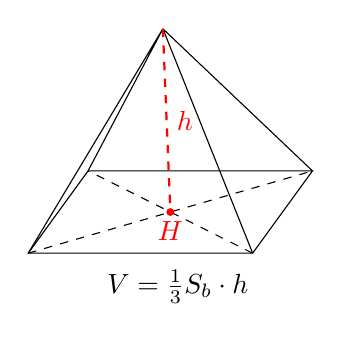
\begin{tikzpicture}[scale=0.95]
  \coordinate (A) at (0,0); \coordinate (B) at (3,0);
  \coordinate (C) at (3.8,1.1); \coordinate (D) at (0.8,1.1);
  \coordinate (S) at (1.8,3.0);
  \draw (A)--(B)--(C)--(D)--cycle;
  \draw (S)--(A) (S)--(B) (S)--(C) (S)--(D);
  \draw[dashed] (A)--(C) (B)--(D);
  \coordinate (H) at (1.9,0.55);
  \draw[dashed,red,thick] (S)--(H) node[midway,right] {$h$};
  \fill[red] (H) circle (1.5pt) node[below] {$H$};
  \node at (2,-0.45) {$V=\frac{1}{3}S_b\cdot h$};
\end{tikzpicture}

\end{document}
